\documentclass[%
 reprint,
%superscriptaddress,
%groupedaddress,
%unsortedaddress,
%runinaddress,
%frontmatterverbose, 
%preprint,
%preprintnumbers,
nofootinbib,
%nobibnotes,
%bibnotes,
 amsmath,amssymb,
 aps,
%pra,
%prb,
%rmp,
%prstab,
%prstper,
%floatfix,
]{revtex4-2}

\usepackage[utf8]{inputenc}
%\usepackage[ngerman]{babel}
\usepackage{booktabs}
\bibliographystyle{unsrt}
\usepackage{graphicx}% Include figure files
\usepackage{dcolumn}% Align table columns on decimal point
\usepackage{bm}% bold math
%\usepackage{hyperref}% add hypertext capabilities
%\usepackage[mathlines]{lineno}% Enable numbering of text and display math
%\linenumbers\relax % Commence numbering lines

%FloatBarrier
\usepackage{placeins}

%\usepackage[showframe,%Uncomment any one of the following lines to test 
%%scale=0.7, marginratio={1:1, 2:3}, ignoreall,% default settings
%%text={7in,10in},centering,
%%margin=1.5in,
%%total={6.5in,8.75in}, top=1.2in, left=0.9in, includefoot,
%%height=10in,a5paper,hmargin={3cm,0.8in},
%]{geometry}
%\usepackage{braket}
\interfootnotelinepenalty=10000
\DeclareUnicodeCharacter{03BD}{}
\DeclareUnicodeCharacter{03C3}{}
\DeclareUnicodeCharacter{03C0}{}
\usepackage{physics}
% Lagrangian command
\newcommand{\Lagr}{\mathcal{L}}

\begin{document}
\preprint{APS/123-QED} 

\title{C$_3$O$_2$(g) necessitates the need to rethink the classical view on molecules}% Force line breaks with \\
%\thanks{A footnote to the article title}%

\author{Konstantin Tamoev}
\author{Markus Antonietti}
\author{Peter E. Bl\"ochl}
\author{Thomas D. K\"uhne}
\email{tkuehne@cp2k.org}
\affiliation{%
Dynamics of Condensed Matter, Chair of Theoretical Chemistry Department, University of Paderborn, Germany
}%

\date{\today}% It is always \today, today,
             %  but any date may be explicitly specified

\begin{abstract}
A chemical and structural analysis of C$_3$O$_2$ on the level of the local hybrid functional PBE0r is presented. For the purpose of reducing the computational complexity and load the Kohn-Sham wave functions are presented in the projector augmented wave formalism. The minimization of the total energy is performed with a Car-Parrinello-like constrained minimization to ensure the orthonormality of the wave functions. Results on this level indicate a deviation from the believed linear structure of C$_3$O$_2$ and agree with prior experimental and theoretical studies. 
\end{abstract}


%\keywords{Suggested keywords}%Use showkeys class option if keyword
                              %display desired
\maketitle

\section{\label{sec:level1} Introduction}
Carbon materials and their multidimensional applications have gained significant interest in recent decades. Ranging from sensor applications, thermal management of optoelectronics, thermal conductivity enhancement, water splitting and $CO_2$ reduction with 2D materials such as graphene \cite{graphene1, graphene2, graphene3, graphene4} and $g-C_3N_4$ \cite{c3n4_1, c3n4_2, c3n4_3} to biomaterial integrated field-effect transistors, biosensors, high capacity hydrogen storage or conductivity enhancement and use as nanoprobes for 3D materials such as carbon nanotubes \cite{cnt1, cnt2, cnt3,cnt4}. Thus, carbonaceous nanomaterials (free of $C-H$ bonds) are key elements in the development of a wide range of applications.

%Analysis of chemical bonds between atoms in a material give insight to its properties. 
In this work, we assess the potential use C$_3$O$_2$, as a carbonaceous material that recently gained renewed interest, by analysing its structural and chemical properties and see whether it can open up the door to a whole new class of (low-temperature) 2D carbonaceous materials. Within the framework of Density Functional Theory (DFT) we propose the use of Crystal Orbital Overlap Populations (COOP) and Density of States (DOS) to gain insight on structrual properties on a chemical level. 

The structure of the paper is as follows. First, we review the methods involved in the use of the local hybrid funcitonal PBE0r in Sec. \ref{methods}. Afterwards, we list the computational details in Sec. \ref{computational_details}. We finish the paper with a discussion of the results in Sec. \ref{results} and giving an outlook for possible future research on the topic in Sec. \ref{conclusions_and_outlook}.
%For this purpose we take a closer look at C$_3$O$_2$, a carbonaceous material that recently gained renewed interest and see whether it can potentially rival the applications of C$_3$N$_4$ and open up the door to a whole new class of (low-temperature) 2D carbonaceous materials. 


\section{\label{methods}Methods}
The Kohn-Sham (KS) method - based on the density functional theory in the local-spin-density approximation (LSDA) - gives insight into the physical and chemical properties\cite{Grechnev_2003} of many materials. To achieve a reduction in the computational complexity and load in solving the KS equations or minimising the DFT energy an efficient representation of the KS wave functions must be used. This is done employing the projector augmented wave formalism\cite{Bloechl1994}. 
%Since a few decades the Kohn-Sham (KS) method, based on the density functional theory (DFT) in the local-spin-density approximation (LSDA) provides a good description of their physical and chemical properties \cite{Grechnev_2003} of many materials. However, the efficient numerical representation of the Kohn-Sham wave functions is of importance for reducing the computational complexity and load in solving the KS equations or minimizing the DFT Energy. We employ here the projector augmented wave formalism (PAW \cite{Bloechl1994}). 
%\textbf{EDIT: Should I give a detailed introduction to PAW as well here?}

%Crystal Orbital Overlap Population (COOP), as first suggested by Hughbanks and Hoffmann \cite{HughbanksAndHoffmann}, and Crystal Orbital Hamilton Poluation (COHP) enable the distinction between bonding and antibonding states, see \ref{COOPsection}.

%The computationally most demanding equation posing numerical difficulties are the one-electron Schrödinger equations, i.e. the KS equations. The calculations were done with the \textit{CP-PAW} code utilizing the Projector Augmented Wave (PAW) formalism. In the PAW formalism \cite{PAW_lda+u} an augmented region $\Omega$, located around the atoms, is introduced and the resulting space outside the augmentation region is called the interstitial region. Near the nuclei the kinetic energy of the electrons is large, resulting in rapid oscillations. A high kinetic energy \cite{HANDSON} in this region makes the Schrödinger equations \textit{stiff}, i.e. a change of the chemical environment, such as the potential, has a negligible effect on the shape of the wavefunction. Outside this region the reverse is true, the kinetic energy is small and the wavefunction is smooth and \textit{flexible},resulting in strong response when the environment is changed. The all-electron (AE) wavefunction with its rapid oscillations near the nuclei and its smoothness in the interstitial regions is constructed from a pseudo (PS) wavefunction and atomic-like functions localized near the nuclei. The AE wavefunction coincides with the PS wavefunction $\ket{\tilde{\Psi}}$ in the interstitial region
%\begin{eqnarray}
%\ket{\Psi(r)}=\ket{\tilde{\Psi}(r)} ~~for ~r \not\in \Omega
%\end{eqnarray}
%and is atomlike in the augmented region. 
\subsection{Car-Parrinello Lagrangian}
Using the Car-Parrinello Lagrangian enables a simultaneous solution of both the classical equations of motion for the atoms and the KS equations for the electrons.
\begin{align}
\Lagr_{\text{CP}} =&& \frac{1}{2}\sum_I^{N_n}M_I\dot{R}_I^2+\frac{1}{2}\mu \sum_i^{N_e}\int d\vb*{r} |\dot{\phi}_i(\vb*{r},t)|^2\nonumber\\
&&-E_{\text{KS}}[{\phi_i},{R_I}] \label{cp_lagrangian}
\end{align}
where E$_{\text{KS}}$ is the Kohn-Sham energy of the system and $\mu$ is the fictitious mass of the wave function. $\mu$ is not a mass in the same sense that $m_e$ is, i.e. $\mu$ is not simply used instead of the electron mass. For one, they have different dimensions as is evident from eqn. (\ref{cp_lagrangian}), [$\mu$]=energy$\cdot$time$^2$. Effectively though, $\mu$ takes on the same role as the mass, which is to say it controls the acceleration of the degrees of freedom of the KS wave functions.
\subsection{Wave Function Dynamics}
Solving the electronic problem to achieve the electronic ground state is done using  \textit{Car-Parrinello Molecular Dynamics}\cite{CP}, i.e. by propagating the orbitals as if they are particles and finding their minimum instead of repeatedly solving the electronic problem. 

The total energy can be expressed as
\begin{eqnarray}
E_{\text{tot}}=&&\sum_nf_n\bra{\dot{\tilde{\Psi}}_n}m_\Psi\ket{\dot{\tilde{\Psi}}_n}+E_{\text{DFT}}\nonumber\\ &&-\sum_{n,m}\bra{\dot{\tilde{\Psi}}_n}\tilde{O}\ket{\dot{\tilde{\Psi}}_m}\Lambda_{n,m}, \label{total_energy}
\end{eqnarray}
with $\tilde{\Psi}$ as the pseudo wave functions of the PAW method, $\Lambda_{n,m}$ as the Lagrange parameters for the wave function orthonormality constraint and 
\begin{eqnarray}
E_{\text{DFT}}&=&\sum_n\bra{\Psi_n}-\frac{1}{2}\Delta^2\ket{\Psi_n} \nonumber\\
&+& \frac{1}{2}\int dr\int dr' \frac{(n(r)+n^Z(r))(n(r')+n^Z(r'))}{|r-r'|} \nonumber\\
&+& \int dr n(r)\epsilon_{xc}(n_\sigma(r), \Delta n_\sigma(r)),
\end{eqnarray}
where $n^Z(r)=-\sum_RZ_R\delta(r-R)$ is the density of the nuclei point charges. 
The minimization of (\ref{total_energy}) is performed with a Car-Parrinello-like constrained minimization to ensure the orthonormality of the wave functions, i.e. $\braket{\psi_n}{\psi_m}=\delta_{i,j}$ and $\sum_if_i=N$, the constraint for the number of particles, have to be fulfilled. 
The equation of motion for the wave functions is
\begin{eqnarray}
m_\Psi\ket{\ddot{\tilde{\Psi}}_n}=-\tilde{H}\ket{\tilde{\Psi}_n}+\sum_m\tilde{O}\Lambda_{m,n}-m_\Psi\dot{\tilde{\Psi}}f_\Psi, \label{equation_of_motion}
\end{eqnarray}
which is solved by discretizing the time coordinate and choosing the Lagrange multipliers in every propagation such that the constraints are fulfilled in the next iteration. 
Here m$_\Psi$ is the fictitious mass of the wave functions. For small values of the kinetic energy of the wave functions the fictitious mass is close to the Born-Oppenheimer surface and thus Eq. (\ref{equation_of_motion}) describes the classical motion of the nuclei. 
\subsection{Damped Nuclear Dynamics}
Minimizing most quantities is done utilizing friction dynamics. Without friction truly dynamical simulations of the atomic structure are performed, while applying friction the system is pushed into the ground state. 
The equation of motion is 
\begin{eqnarray}
m\ddot{x} = F(x) - m\alpha \dot{x}, \label{nuclei_equation_of_motion}
\end{eqnarray}
where the mass has been integrated into the friction coefficient, $m\alpha$. Discretizing Eq. (\ref{nuclei_equation_of_motion}) using the Verlet\cite{Verlet} algorithm and setting $a=\frac{\alpha\Delta}{2}$ the equation of motion can be written as 
\begin{eqnarray}
x(t+\Delta)=&\frac{2}{1+a}x(t)-\frac{1-a}{1+a}x(t-\Delta)&\nonumber\\ &+\frac{1}{m}F(x)\frac{\Delta^2}{1+a}&\label{new_fric}
\end{eqnarray}
Setting $a=0$, i.e. undamped dynamics, Eq. (\ref{new_fric}) results in the original Verlet algorithm
\begin{eqnarray}
x(t+\Delta)=2x(t)-x(t-\Delta)+\frac{1}{m}F(x)\Delta^2, \label{original_verlet}
\end{eqnarray}
whose dynamics over long time scales is energy conserving and independent of the step size due to time inversion symmetry. 
The steepest descent is given by $a=1$:
\begin{eqnarray}
x(t+\Delta)=x(t)-\frac{1}{m}F(x)\frac{\Delta^2}{2}, \label{steepest_descent}
\end{eqnarray}
with $\frac{\Delta^2}{2m}$ as the mixing parameter. While Eq. (\ref{steepest_descent}) describes a dynamics with infinite friction, the motion does not come to rest in this limit because the time step is scaled inversely proportional. \cite{CPPAWMANUAL}

\subsection{\label{COOPsection} How to analyse bonds}
The band structure energy is defined as 
\begin{eqnarray}
E_\text{B} =\sum_n f_n\epsilon_n \label{bandenergy_initial}
\end{eqnarray}
where $\epsilon_n$ are the orbital energies and $f_n$ the corresponding occupations. Eq. \ref{bandenergy_initial} can also be written in terms of the density of states\cite{HANDSON}(\textbf{FIX citation})
\begin{eqnarray}
E_\text{B}&=&\int_{-\infty}^{\infty}d\epsilon f(\epsilon-\mu)\epsilon\sum_n\delta(\epsilon-\epsilon_n)\\
&=&\int_{-\infty}^{\infty}d\epsilon D(\epsilon)\epsilon f(\epsilon-\mu), \label{bandenergy}
\end{eqnarray}
where $f$ refers to the fermi-distribution. At T=0 the chemical potential is the Fermi Energy of the system and lies between the highest occupied and lowest unoccupied state. 
Density of States give insights into the binding properties of materials in a local and energy resolved manner.

Using projector functions the wave functions can be decomposed into local orbitals\footnote{Which can be non-orthogonal.} $\chi_i$ \cite{Bloechl1994}
\begin{eqnarray}
\ket{\psi_n}=\sum_i\ket{\chi_i}\bra{p_i}\ket{\psi_n} \label{wave_functions_by_local_orbitals}
\end{eqnarray}
For this to hold the basis functions must be completed and mutually orthonormal with the projector functions.
Assuming the wave functions are normalized and using eq. (\ref{wave_functions_by_local_orbitals}) total DOS D($\epsilon$) can be expressed by a local basis set

\begin{eqnarray}
&&\sum_n\delta(\epsilon-\epsilon_n)\bra{\psi_n}\ket{\psi_n}\nonumber\\
&&=\sum_{i,j}\sum_n\delta(\epsilon-\epsilon_n)\bra{\psi_n}\ket{p_i}\bra{\chi_i}\ket{\chi_j}\bra{p_j}\ket{\psi_n}\nonumber\\
&&=\sum_{i,j}D_{j,i}(\epsilon)\bra{\chi_i}\ket{\chi_j} \label{local_basis_dos}
\end{eqnarray}

The diagonal elements $D_{j,j}\bra{\chi_j}\ket{\chi_j}$ are called the \textit{projected density of states}\cite{HANDSON}(\textbf{Fix citation}). The off-diagonal elements, or the hopping terms, are the Crystal Orbital Overlap Populations \cite{HughbanksAndHoffmann}. 
The COOPs give an additional layer of information by providing insight into the bonding information. Positive values indicate a charge accumulation in the bond, \textit{bonding} states, while negative values indicate antibonding states. The sum of the overlap population over all states is a measure for the strength of the bond. 
However, COOPs are basis set dependent quantities and thus in general are no absolute bonding indicators.
\hfill\break Strictly speaking the COOPs do not contribute to the total energy of the system. 
Multiplying Eq. (\ref{local_basis_dos}) by the energy we have
\begin{eqnarray}
D(\epsilon)\epsilon &=&\sum_n\delta(\epsilon-\epsilon_n)\epsilon\bra{\psi_n}\ket{\psi_n} \nonumber\\
&=&\sum_n\delta(\epsilon-\epsilon_n)\epsilon\bra{\psi_n}\hat{H}\ket{\psi_n} \nonumber\\
&=&\sum_{i,j}\sum_n\delta(\epsilon-\epsilon_n)\bra{\psi_n}\ket{p_i}\nonumber\\
&\cdot&\bra{\chi_i}\hat{H}\ket{\chi_j}\bra{p_j}\ket{\psi_n} \nonumber\\
&=&D_{j,i}(\epsilon)\bra{\chi_i}\hat{H}\ket{\chi_j} \label{COHP}
\end{eqnarray}
where the last term in (\ref{COHP}) is the \textit{Crystal Orbital Hamilton Population}(COHP)\cite{dronskowski1993crystal}. Eq. (\ref{COHP}) contains information about bonding, nonbonding and antibonding energy regions within a specified energy range, while integrating the COHP reveals the contributions of an atom or bond to the distribution of one-particle energies\cite{dronskowski1993crystal}. The sign convention is opposite to that of the COOPs, i.e. bonding states are negative off-site terms and antibonding states are positive. 

\section{\label{computational_details}Computational Details}
Calculations were done with the local hybrid functional PBE0r by Blöchl et. al. \cite{BloechlLocal} that is based on the PBE0 \cite{PBE0} functional. In the latter a fraction of the PBE exchange energy $E_x^{\text{PBE}}$ is replaced by the explicit non-local HF exchange energy $E_x^{\text{HF}}$, i.e.:
\begin{eqnarray}
E^{\text{PBE0}}=E^{\text{PBE}} + a_x(E_x^{\text{HF}}-E_x^{\text{PBE}})
\end{eqnarray}
The Kohn-Sham wave functions in the PBE0r are mapped onto local tight-binding orbitals (LTBO) and the off-site terms are excluded from the exchange correction. This restriction on the exchange correction enables a sort of range separation bearing similarities to the long-range screening of the interaction in the $GW$ approximation. 
This exclusion of off-site terms is appropriate for materials such as transition metal oxides which have strongly localized $d$ orbitals whereas it is not suitable for the description of systems containing strong covalent bonds. \cite{BloechlLocal}
The admixture $a_x$\cite{PerdewPBE0, BloechlLocal} is a freely adjustable parameter in PBE0r and can be set to fit experimentally observed spectral features. The mixing parameter can be chosen individually for each atom and thus, essentially, describes a local dielectric constant. 
Calculations are done in a 15$\times$15$\times$15 unit cell, the plane wave cutoff value for the wave functions is set to 30Ry and the contribution of the non-local HF exchange energy set to 10\%.


\section{\label{results}Results and Discussion}
%\begin{figure}[t]
%\center
%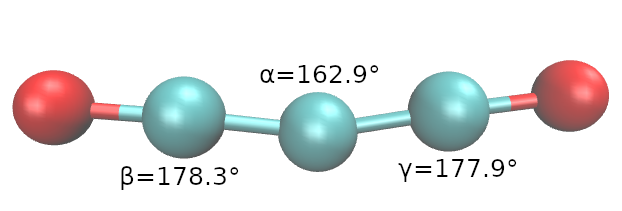
\includegraphics[scale=0.34]{structure_angles.png}
%\caption{C3O2 structure \label{c3o2_structure}}
%\end{figure}

Figure \ref{single_point_calculations} shows the single point energies of both PBE and PBE0r at different angles $\alpha$(C-C-C). 
While PBE results indicate a clear linear structure for C$_3$O$_2$, PBE0r results have an energetic minium  at around 170$^\circ$, indicating that the molecule has a slight bent around its center Carbon atom.
%In general both functionals have a similar energetic decrease towards 180$^\circ$. However, while PBE results indicate a preferred linear structure of C$_3$O$_2$, PBE0r reveals a minimum in energy at around 170$^\circ$ and thus preferring a slightly bent geometry for the molecule. 

As discussed in sec. \ref{COOPsection} the off-site terms of the overlap matrix give insight into the electron correlation and chemical bonding properties of materials and as such also to the physics and chemistry that lead to the bent structure.

Figure \ref{dos_separated} shows the total DOS as well as the projected DOS of the individual orbitals for Oxygen and Carbon.
While the mixed state at -30eV has contributions from the Carbon $s$ and $p$ orbitals, it exhibits a predominant Oxygen $s$ character. 
The state at -22eV can be identified as a bonding state between the $s$ orbital of the center Carbon atom with the $s$ and $p$ orbitals of the two neighbouring Carbon atoms. Analogously, the state at -18eV is the mixed antibonding state between the $p$ orbitals of the center Carbon with the $s$ and $p$ orbitals of its neighbours. The orbital character in both states is dominated by the contribution from the central Carbon, i.e. the states at -22eV and -18eV are of primarily $s$ and $p$ character, respectively. The final state before the Fermi Energy starting at [-13eV,-11] is a bonding state between the $p$ orbitals of both Oxygen and the two outer Carbons. 

The projected DOS of both atom types approximately shows an energetic separation of the $s$ and $p$ orbitals at lower energies, while this is not the case for states above $\approx$-13eV and close to the Fermi Energy.
\begin{figure}
    \centering
     \includegraphics[scale=0.36]{bent_wings.eps}
    \caption{Single point calculations with PBE and PBE0r.\label{single_point_calculations}}
    \label{shorter_oc_bond}
\end{figure}
%\begin{figure}
%    \centering
%    \includegraphics[scale=0.36]{energies_mc4.eps}
%    \caption{LRDMC and VMC calculations.}
%    \label{energies_mc}
%\end{figure}

\begin{figure}[t]
\includegraphics[scale=0.35]{dos_final.png}
\caption{First row: Total DOS including projected DOS of oxygen $s$, $p$ and carbon $s$, $p$ orbitals (due to negligible contribution of $d$ orbitals to the total DOS these were not included in the DOS calculations). Second and Third Row: Projected DOS of oxygen and carbon, respectively. Fourth Row: Bonding (orange) and antibonding (red) states. Fifth and Sixth Row: COOP for the $p$ contribution of the $O-C$ and $C-C$ bond, respectively. Note: \textit{inner} here refers to contributions from the center Carbon atom and \textit{outer} to the two neighbouring Carbon atoms. \label{dos_separated}}
\end{figure}

%\begin{figure}
%    \centering
%    \includegraphics[scale=0.36]{straight_wings.eps}
%    \caption{Single point calculations for $O-C$ bond lengths of 1.44 Angström.}
%    \label{longer_oc_bond}
%\end{figure}

The COOP for the O-C and C-C bonds show strong $p$-contributions, indicating the formation of $pp_\pi$-bonds. This is further confirmed by the \textit{highest occupied molecular orbital}(HOMO) in Fig. \ref{HOMO} whose orbitals are perpendicular to the given bond directions, indicative of $pp_\pi$-bonds. 

\begin{figure}
    \centering
    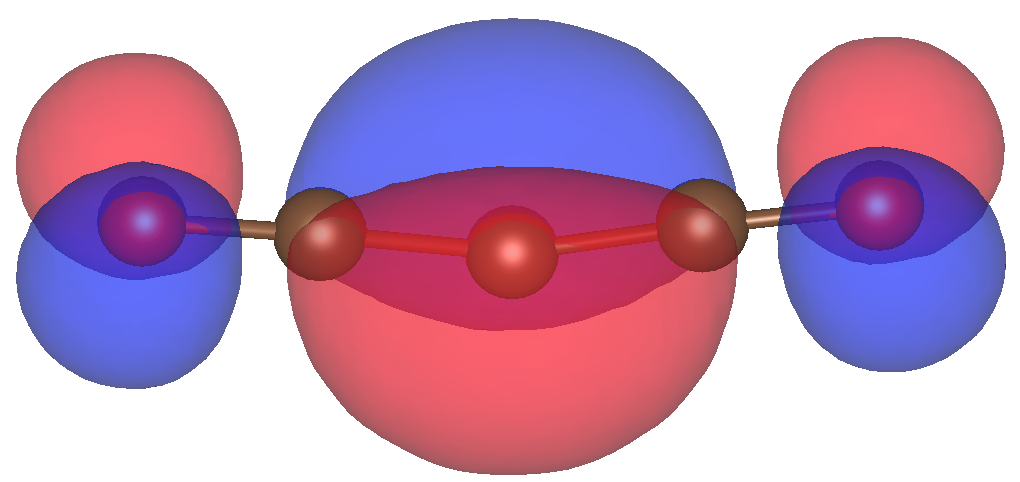
\includegraphics[scale=0.23]{homo3.png}
    \caption{HOMO of the $C_3O_2$. Contour and mesh plots of the HOMO are given in the supplementary figures.}
    \label{HOMO}
\end{figure}

The valence state at the Fermi level, see Fig. \ref{dos_separated}, contains contributions of $p$ orbitals of both Oxygen and Carbon. The contribution from the central Carbon to the valence state is significantly higher than that of its neighbours and is similar to that of the Oxygen. The partial charge on the center Carbon was calculated to be -0.23e. According to the VSEPR\cite{VSEPR} theory this partial charge will exhibit a repulsive force on the neighbours of the Carbon and can thus explain the slight bent that is preferred when using the local hybrid funcitonal and which coincides with prior experimental and theoretical studies\cite{Tortajada, VanderJohns, Jensen,Koput,HimmelKrossingSchnepf}. 


\section{\label{conclusions_and_outlook}Conclusions and Outlook}

We have shown that the carbon suboxide in the gas phase minimizes into a bent geometry. This result conforms with calculations with higher-level methods but was achieved on a computationally much less demanding scope. 

The bent structure goes contrary to our intuitive understanding of even such an apparently simple molecule. Not only does this suggest that C$_3$O$_2$ might exhibit the same properties as $g-C_3N_4$ does, e.g. for instance the possibility to synthesize C$_3$O$_2$ into a graphene-like substance, but it also opens up the possibility to gain new insight from other "ordinary" molecules and compounds from old chemistry that may have been overlooked due to our now seemingly faulty chemical intuition. Hopefully the present results are incentive enough to include some of the few hundred years of old chemical knowledge into future research and make new from old. 


\FloatBarrier
\nocite{*}
\bibliography{references}
\end{document}